\documentclass[12pt,letterpaper]{article}
\usepackage[T1]{fontenc}
\usepackage{tgheros}
\renewcommand{\familydefault}{\sfdefault}
\usepackage[letterpaper, left=0.75in, right=0.75in, top=0.85in, bottom=0.85in,
  headheight=16pt, headsep=14pt, footskip=26pt]{geometry}
\usepackage{fancyhdr}
\usepackage{pifont}
\usepackage{tikz}
\usetikzlibrary{arrows.meta}
\pagestyle{fancy}
\fancyhf{}
\fancyhead[L]{Week NN / Train-yard sorting / Grades 2–3}
\fancyfoot[L]{\small Bellingham Math Circle / Week NN / TY-23-v1}
\fancyfoot[R]{\small \thepage}
\renewcommand{\headrulewidth}{0.4pt}
\renewcommand{\footrulewidth}{0pt}
\setlength{\parindent}{0pt}
\setlength{\parskip}{4pt}
\newcommand{\problem}[1]{\par\vspace{14pt}\noindent\textbf{Problem #1:} }
\newcommand{\yes}{\ding{51}}
\newcommand{\no}{\ding{55}}
\begin{document}

Put a train on the arrival track exactly as it is drawn, so the car on the left arrives first. Each move sends the front car of the arrival track down into the siding, or sends the top car of the siding out to the departure track. Cars slide along the table and never jump over each other. A car in the siding cannot go back to the arrival track. A train can \emph{leave in order} if its cars can reach the departure track in the order 1, 2, 3, and so on.

\par\vspace{2pt}\begin{center}
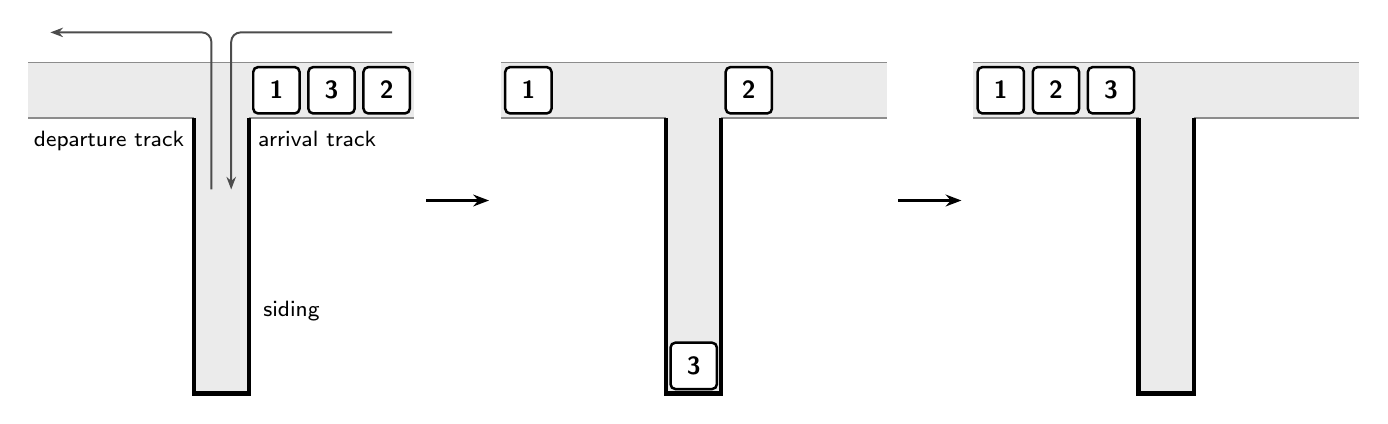
\begin{tikzpicture}[x=1mm,y=1mm]
\begin{scope}[shift={(21,0)}]
\fill[black!8] (-21,0) rectangle (28,7);
\fill[black!8] (0,-35) rectangle (7,0);
\draw[black!45, line width=0.5pt] (-21,7) -- (28,7);
\draw[black!45, line width=0.5pt] (-21,0) -- (0,0);
\draw[black!45, line width=0.5pt] (7,0) -- (28,0);
\draw[line width=1.6pt] (0,0) -- (0,-35) -- (7,-35) -- (7,0);
\draw[line width=0.9pt, fill=white, rounded corners=0.6mm] (7.56,0.56) rectangle (13.44,6.44);
\node at (10.5,3.5) {\bfseries\small 1};
\draw[line width=0.9pt, fill=white, rounded corners=0.6mm] (14.56,0.56) rectangle (20.44,6.44);
\node at (17.5,3.5) {\bfseries\small 3};
\draw[line width=0.9pt, fill=white, rounded corners=0.6mm] (21.56,0.56) rectangle (27.44,6.44);
\node at (24.5,3.5) {\bfseries\small 2};
\node[font=\footnotesize, below left, inner xsep=1pt] at (-0.8,-0.4) {departure track};
\node[font=\footnotesize, below right, inner xsep=1pt] at (7.8,-0.4) {arrival track};
\node[font=\footnotesize, right] at (7.6,-24.5) {siding};
\draw[-{Stealth[length=1.6mm]}, line width=0.7pt, black!70, rounded corners=1.2mm] (25.2,10.85) -- (4.76,10.85) -- (4.76,-9.1);
\draw[-{Stealth[length=1.6mm]}, line width=0.7pt, black!70, rounded corners=1.2mm] (2.24,-9.1) -- (2.24,10.85) -- (-18.2,10.85);
\end{scope}
\draw[-{Stealth[length=2mm]}, line width=0.9pt] (50.5,-10.5) -- (58.5,-10.5);
\begin{scope}[shift={(81,0)}]
\fill[black!8] (-21,0) rectangle (28,7);
\fill[black!8] (0,-35) rectangle (7,0);
\draw[black!45, line width=0.5pt] (-21,7) -- (28,7);
\draw[black!45, line width=0.5pt] (-21,0) -- (0,0);
\draw[black!45, line width=0.5pt] (7,0) -- (28,0);
\draw[line width=1.6pt] (0,0) -- (0,-35) -- (7,-35) -- (7,0);
\draw[line width=0.9pt, fill=white, rounded corners=0.6mm] (-20.44,0.56) rectangle (-14.56,6.44);
\node at (-17.5,3.5) {\bfseries\small 1};
\draw[line width=0.9pt, fill=white, rounded corners=0.6mm] (0.56,-34.44) rectangle (6.44,-28.56);
\node at (3.5,-31.5) {\bfseries\small 3};
\draw[line width=0.9pt, fill=white, rounded corners=0.6mm] (7.56,0.56) rectangle (13.44,6.44);
\node at (10.5,3.5) {\bfseries\small 2};
\end{scope}
\draw[-{Stealth[length=2mm]}, line width=0.9pt] (110.5,-10.5) -- (118.5,-10.5);
\begin{scope}[shift={(141,0)}]
\fill[black!8] (-21,0) rectangle (28,7);
\fill[black!8] (0,-35) rectangle (7,0);
\draw[black!45, line width=0.5pt] (-21,7) -- (28,7);
\draw[black!45, line width=0.5pt] (-21,0) -- (0,0);
\draw[black!45, line width=0.5pt] (7,0) -- (28,0);
\draw[line width=1.6pt] (0,0) -- (0,-35) -- (7,-35) -- (7,0);
\draw[line width=0.9pt, fill=white, rounded corners=0.6mm] (-20.44,0.56) rectangle (-14.56,6.44);
\node at (-17.5,3.5) {\bfseries\small 1};
\draw[line width=0.9pt, fill=white, rounded corners=0.6mm] (-13.44,0.56) rectangle (-7.56,6.44);
\node at (-10.5,3.5) {\bfseries\small 2};
\draw[line width=0.9pt, fill=white, rounded corners=0.6mm] (-6.44,0.56) rectangle (-0.56,6.44);
\node at (-3.5,3.5) {\bfseries\small 3};
\end{scope}
\end{tikzpicture}
\end{center}

\problem{1}Write every different train you can make with cars 1, 2, 3. Mark each one \yes{} if it can leave in order and \no{} if it cannot.
\par\vspace{8pt}\begin{center}
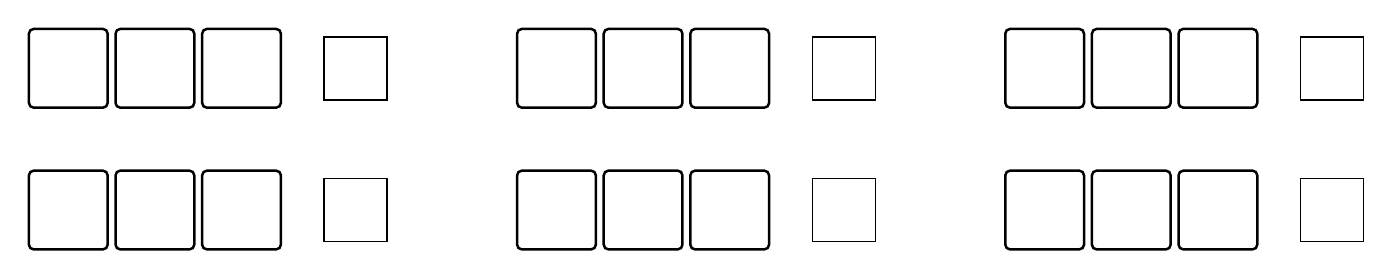
\begin{tikzpicture}[x=1mm,y=1mm]
\draw[line width=0.9pt, fill=white, rounded corners=0.6mm] (0,0) rectangle (10,10);
\draw[line width=0.9pt, fill=white, rounded corners=0.6mm] (11,0) rectangle (21,10);
\draw[line width=0.9pt, fill=white, rounded corners=0.6mm] (22,0) rectangle (32,10);
\draw[line width=0.6pt] (37.5,1) rectangle (45.5,9);
\draw[line width=0.9pt, fill=white, rounded corners=0.6mm] (62,0) rectangle (72,10);
\draw[line width=0.9pt, fill=white, rounded corners=0.6mm] (73,0) rectangle (83,10);
\draw[line width=0.9pt, fill=white, rounded corners=0.6mm] (84,0) rectangle (94,10);
\draw[line width=0.6pt] (99.5,1) rectangle (107.5,9);
\draw[line width=0.9pt, fill=white, rounded corners=0.6mm] (124,0) rectangle (134,10);
\draw[line width=0.9pt, fill=white, rounded corners=0.6mm] (135,0) rectangle (145,10);
\draw[line width=0.9pt, fill=white, rounded corners=0.6mm] (146,0) rectangle (156,10);
\draw[line width=0.6pt] (161.5,1) rectangle (169.5,9);
\draw[line width=0.9pt, fill=white, rounded corners=0.6mm] (0,-18) rectangle (10,-8);
\draw[line width=0.9pt, fill=white, rounded corners=0.6mm] (11,-18) rectangle (21,-8);
\draw[line width=0.9pt, fill=white, rounded corners=0.6mm] (22,-18) rectangle (32,-8);
\draw[line width=0.6pt] (37.5,-17) rectangle (45.5,-9);
\draw[line width=0.9pt, fill=white, rounded corners=0.6mm] (62,-18) rectangle (72,-8);
\draw[line width=0.9pt, fill=white, rounded corners=0.6mm] (73,-18) rectangle (83,-8);
\draw[line width=0.9pt, fill=white, rounded corners=0.6mm] (84,-18) rectangle (94,-8);
\draw[line width=0.6pt] (99.5,-17) rectangle (107.5,-9);
\draw[line width=0.9pt, fill=white, rounded corners=0.6mm] (124,-18) rectangle (134,-8);
\draw[line width=0.9pt, fill=white, rounded corners=0.6mm] (135,-18) rectangle (145,-8);
\draw[line width=0.9pt, fill=white, rounded corners=0.6mm] (146,-18) rectangle (156,-8);
\draw[line width=0.6pt] (161.5,-17) rectangle (169.5,-9);
\end{tikzpicture}
\end{center}

\newpage
\problem{2}Cars 1, 2, 3, 4 can be lined up as 24 different trains. With the other pair at your table, write each of these trains on a card, drive it, and sort the cards into a pile of trains that can leave in order and a pile of trains that cannot. How many cards are in each pile?
\par\vspace{14pt}\hspace*{1.5em}Can leave in order: \rule{2.2cm}{0.5pt}\hspace{3em}Cannot: \rule{2.2cm}{0.5pt}
\vspace{18pt}
\problem{3}Which of these trains can leave in order? Mark each one \yes{} or \no.
\par\vspace{8pt}\begin{center}
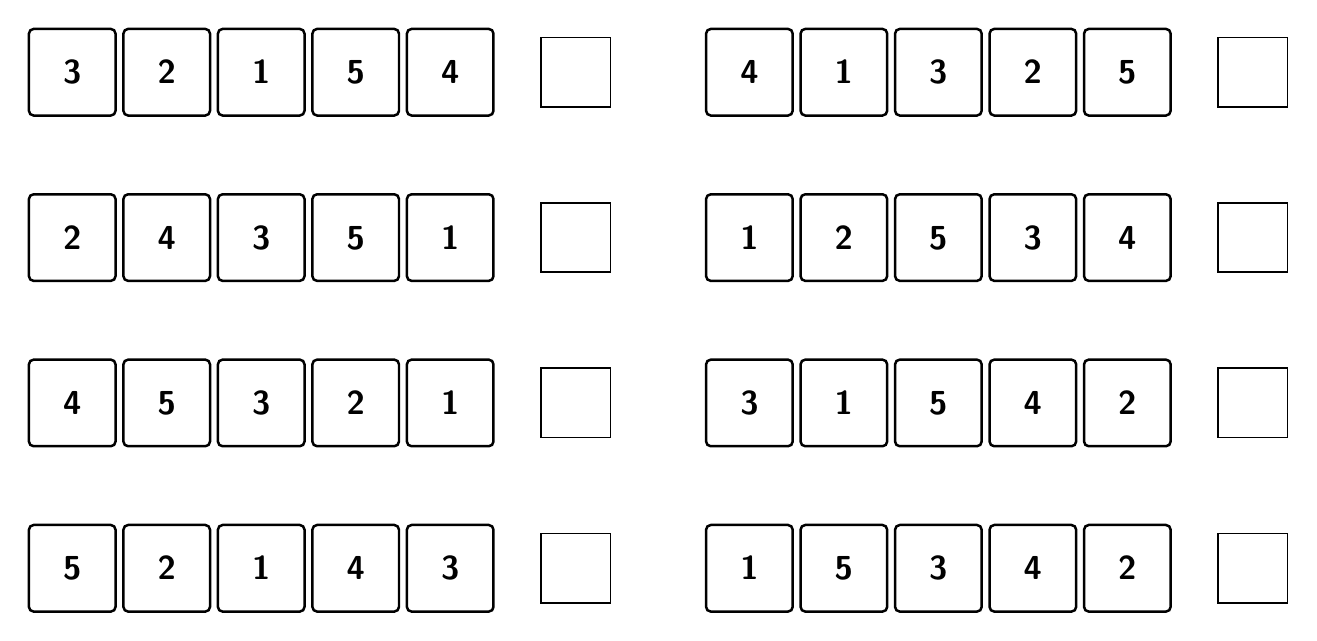
\begin{tikzpicture}[x=1mm,y=1mm]
\draw[line width=0.9pt, fill=white, rounded corners=0.6mm] (0,0) rectangle (11,11);
\node at (5.5,5.5) {\bfseries\large 3};
\draw[line width=0.9pt, fill=white, rounded corners=0.6mm] (12,0) rectangle (23,11);
\node at (17.5,5.5) {\bfseries\large 2};
\draw[line width=0.9pt, fill=white, rounded corners=0.6mm] (24,0) rectangle (35,11);
\node at (29.5,5.5) {\bfseries\large 1};
\draw[line width=0.9pt, fill=white, rounded corners=0.6mm] (36,0) rectangle (47,11);
\node at (41.5,5.5) {\bfseries\large 5};
\draw[line width=0.9pt, fill=white, rounded corners=0.6mm] (48,0) rectangle (59,11);
\node at (53.5,5.5) {\bfseries\large 4};
\draw[line width=0.6pt] (65.05,1.1) rectangle (73.85,9.9);
\draw[line width=0.9pt, fill=white, rounded corners=0.6mm] (86,0) rectangle (97,11);
\node at (91.5,5.5) {\bfseries\large 4};
\draw[line width=0.9pt, fill=white, rounded corners=0.6mm] (98,0) rectangle (109,11);
\node at (103.5,5.5) {\bfseries\large 1};
\draw[line width=0.9pt, fill=white, rounded corners=0.6mm] (110,0) rectangle (121,11);
\node at (115.5,5.5) {\bfseries\large 3};
\draw[line width=0.9pt, fill=white, rounded corners=0.6mm] (122,0) rectangle (133,11);
\node at (127.5,5.5) {\bfseries\large 2};
\draw[line width=0.9pt, fill=white, rounded corners=0.6mm] (134,0) rectangle (145,11);
\node at (139.5,5.5) {\bfseries\large 5};
\draw[line width=0.6pt] (151.05,1.1) rectangle (159.85,9.9);
\draw[line width=0.9pt, fill=white, rounded corners=0.6mm] (0,-21) rectangle (11,-10);
\node at (5.5,-15.5) {\bfseries\large 2};
\draw[line width=0.9pt, fill=white, rounded corners=0.6mm] (12,-21) rectangle (23,-10);
\node at (17.5,-15.5) {\bfseries\large 4};
\draw[line width=0.9pt, fill=white, rounded corners=0.6mm] (24,-21) rectangle (35,-10);
\node at (29.5,-15.5) {\bfseries\large 3};
\draw[line width=0.9pt, fill=white, rounded corners=0.6mm] (36,-21) rectangle (47,-10);
\node at (41.5,-15.5) {\bfseries\large 5};
\draw[line width=0.9pt, fill=white, rounded corners=0.6mm] (48,-21) rectangle (59,-10);
\node at (53.5,-15.5) {\bfseries\large 1};
\draw[line width=0.6pt] (65.05,-19.9) rectangle (73.85,-11.1);
\draw[line width=0.9pt, fill=white, rounded corners=0.6mm] (86,-21) rectangle (97,-10);
\node at (91.5,-15.5) {\bfseries\large 1};
\draw[line width=0.9pt, fill=white, rounded corners=0.6mm] (98,-21) rectangle (109,-10);
\node at (103.5,-15.5) {\bfseries\large 2};
\draw[line width=0.9pt, fill=white, rounded corners=0.6mm] (110,-21) rectangle (121,-10);
\node at (115.5,-15.5) {\bfseries\large 5};
\draw[line width=0.9pt, fill=white, rounded corners=0.6mm] (122,-21) rectangle (133,-10);
\node at (127.5,-15.5) {\bfseries\large 3};
\draw[line width=0.9pt, fill=white, rounded corners=0.6mm] (134,-21) rectangle (145,-10);
\node at (139.5,-15.5) {\bfseries\large 4};
\draw[line width=0.6pt] (151.05,-19.9) rectangle (159.85,-11.1);
\draw[line width=0.9pt, fill=white, rounded corners=0.6mm] (0,-42) rectangle (11,-31);
\node at (5.5,-36.5) {\bfseries\large 4};
\draw[line width=0.9pt, fill=white, rounded corners=0.6mm] (12,-42) rectangle (23,-31);
\node at (17.5,-36.5) {\bfseries\large 5};
\draw[line width=0.9pt, fill=white, rounded corners=0.6mm] (24,-42) rectangle (35,-31);
\node at (29.5,-36.5) {\bfseries\large 3};
\draw[line width=0.9pt, fill=white, rounded corners=0.6mm] (36,-42) rectangle (47,-31);
\node at (41.5,-36.5) {\bfseries\large 2};
\draw[line width=0.9pt, fill=white, rounded corners=0.6mm] (48,-42) rectangle (59,-31);
\node at (53.5,-36.5) {\bfseries\large 1};
\draw[line width=0.6pt] (65.05,-40.9) rectangle (73.85,-32.1);
\draw[line width=0.9pt, fill=white, rounded corners=0.6mm] (86,-42) rectangle (97,-31);
\node at (91.5,-36.5) {\bfseries\large 3};
\draw[line width=0.9pt, fill=white, rounded corners=0.6mm] (98,-42) rectangle (109,-31);
\node at (103.5,-36.5) {\bfseries\large 1};
\draw[line width=0.9pt, fill=white, rounded corners=0.6mm] (110,-42) rectangle (121,-31);
\node at (115.5,-36.5) {\bfseries\large 5};
\draw[line width=0.9pt, fill=white, rounded corners=0.6mm] (122,-42) rectangle (133,-31);
\node at (127.5,-36.5) {\bfseries\large 4};
\draw[line width=0.9pt, fill=white, rounded corners=0.6mm] (134,-42) rectangle (145,-31);
\node at (139.5,-36.5) {\bfseries\large 2};
\draw[line width=0.6pt] (151.05,-40.9) rectangle (159.85,-32.1);
\draw[line width=0.9pt, fill=white, rounded corners=0.6mm] (0,-63) rectangle (11,-52);
\node at (5.5,-57.5) {\bfseries\large 5};
\draw[line width=0.9pt, fill=white, rounded corners=0.6mm] (12,-63) rectangle (23,-52);
\node at (17.5,-57.5) {\bfseries\large 2};
\draw[line width=0.9pt, fill=white, rounded corners=0.6mm] (24,-63) rectangle (35,-52);
\node at (29.5,-57.5) {\bfseries\large 1};
\draw[line width=0.9pt, fill=white, rounded corners=0.6mm] (36,-63) rectangle (47,-52);
\node at (41.5,-57.5) {\bfseries\large 4};
\draw[line width=0.9pt, fill=white, rounded corners=0.6mm] (48,-63) rectangle (59,-52);
\node at (53.5,-57.5) {\bfseries\large 3};
\draw[line width=0.6pt] (65.05,-61.9) rectangle (73.85,-53.1);
\draw[line width=0.9pt, fill=white, rounded corners=0.6mm] (86,-63) rectangle (97,-52);
\node at (91.5,-57.5) {\bfseries\large 1};
\draw[line width=0.9pt, fill=white, rounded corners=0.6mm] (98,-63) rectangle (109,-52);
\node at (103.5,-57.5) {\bfseries\large 5};
\draw[line width=0.9pt, fill=white, rounded corners=0.6mm] (110,-63) rectangle (121,-52);
\node at (115.5,-57.5) {\bfseries\large 3};
\draw[line width=0.9pt, fill=white, rounded corners=0.6mm] (122,-63) rectangle (133,-52);
\node at (127.5,-57.5) {\bfseries\large 4};
\draw[line width=0.9pt, fill=white, rounded corners=0.6mm] (134,-63) rectangle (145,-52);
\node at (139.5,-57.5) {\bfseries\large 2};
\draw[line width=0.6pt] (151.05,-61.9) rectangle (159.85,-53.1);
\end{tikzpicture}
\end{center}

\newpage
\problem{4}What makes a train impossible? Write a way to tell, without driving the cars, whether a train can leave in order.
\par\vspace{3pt}\noindent\begin{tikzpicture}[x=1mm,y=1mm]
\draw[black!30, line width=0.4pt] (0,-9) -- (177,-9);
\draw[black!30, line width=0.4pt] (0,-18) -- (177,-18);
\draw[black!30, line width=0.4pt] (0,-27) -- (177,-27);
\draw[black!30, line width=0.4pt] (0,-36) -- (177,-36);
\draw[black!30, line width=0.4pt] (0,-45) -- (177,-45);
\draw[black!30, line width=0.4pt] (0,-54) -- (177,-54);
\draw[black!30, line width=0.4pt] (0,-63) -- (177,-63);
\draw[black!30, line width=0.4pt] (0,-72) -- (177,-72);
\end{tikzpicture}\par
\vspace{10pt}
\problem{5}Decide without driving which of these trains can leave in order, and mark each one \yes{} or \no. Then drive them to check.
\par\vspace{8pt}\begin{center}
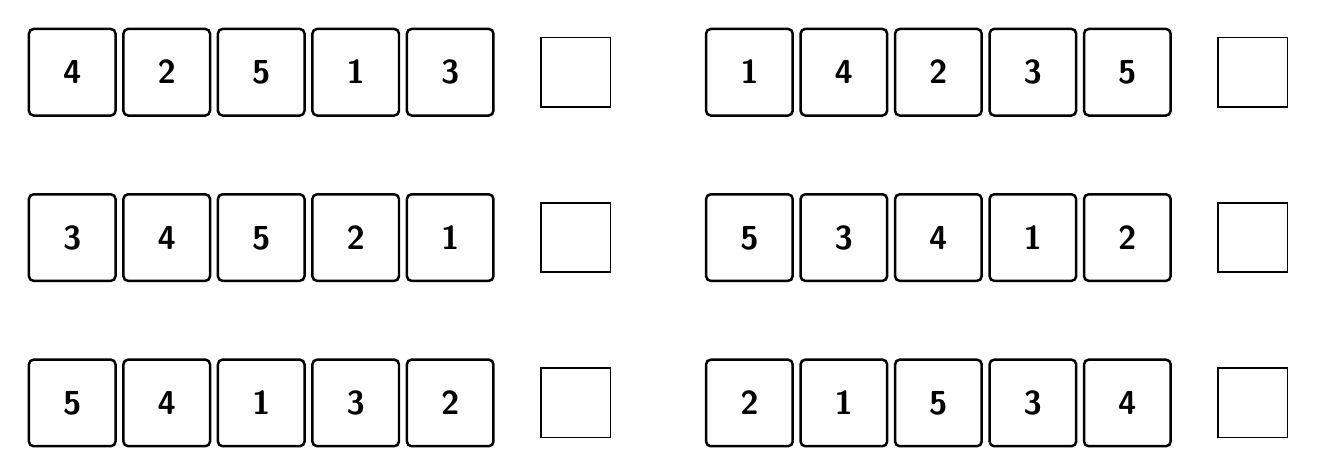
\begin{tikzpicture}[x=1mm,y=1mm]
\draw[line width=0.9pt, fill=white, rounded corners=0.6mm] (0,0) rectangle (11,11);
\node at (5.5,5.5) {\bfseries\large 4};
\draw[line width=0.9pt, fill=white, rounded corners=0.6mm] (12,0) rectangle (23,11);
\node at (17.5,5.5) {\bfseries\large 2};
\draw[line width=0.9pt, fill=white, rounded corners=0.6mm] (24,0) rectangle (35,11);
\node at (29.5,5.5) {\bfseries\large 5};
\draw[line width=0.9pt, fill=white, rounded corners=0.6mm] (36,0) rectangle (47,11);
\node at (41.5,5.5) {\bfseries\large 1};
\draw[line width=0.9pt, fill=white, rounded corners=0.6mm] (48,0) rectangle (59,11);
\node at (53.5,5.5) {\bfseries\large 3};
\draw[line width=0.6pt] (65.05,1.1) rectangle (73.85,9.9);
\draw[line width=0.9pt, fill=white, rounded corners=0.6mm] (86,0) rectangle (97,11);
\node at (91.5,5.5) {\bfseries\large 1};
\draw[line width=0.9pt, fill=white, rounded corners=0.6mm] (98,0) rectangle (109,11);
\node at (103.5,5.5) {\bfseries\large 4};
\draw[line width=0.9pt, fill=white, rounded corners=0.6mm] (110,0) rectangle (121,11);
\node at (115.5,5.5) {\bfseries\large 2};
\draw[line width=0.9pt, fill=white, rounded corners=0.6mm] (122,0) rectangle (133,11);
\node at (127.5,5.5) {\bfseries\large 3};
\draw[line width=0.9pt, fill=white, rounded corners=0.6mm] (134,0) rectangle (145,11);
\node at (139.5,5.5) {\bfseries\large 5};
\draw[line width=0.6pt] (151.05,1.1) rectangle (159.85,9.9);
\draw[line width=0.9pt, fill=white, rounded corners=0.6mm] (0,-21) rectangle (11,-10);
\node at (5.5,-15.5) {\bfseries\large 3};
\draw[line width=0.9pt, fill=white, rounded corners=0.6mm] (12,-21) rectangle (23,-10);
\node at (17.5,-15.5) {\bfseries\large 4};
\draw[line width=0.9pt, fill=white, rounded corners=0.6mm] (24,-21) rectangle (35,-10);
\node at (29.5,-15.5) {\bfseries\large 5};
\draw[line width=0.9pt, fill=white, rounded corners=0.6mm] (36,-21) rectangle (47,-10);
\node at (41.5,-15.5) {\bfseries\large 2};
\draw[line width=0.9pt, fill=white, rounded corners=0.6mm] (48,-21) rectangle (59,-10);
\node at (53.5,-15.5) {\bfseries\large 1};
\draw[line width=0.6pt] (65.05,-19.9) rectangle (73.85,-11.1);
\draw[line width=0.9pt, fill=white, rounded corners=0.6mm] (86,-21) rectangle (97,-10);
\node at (91.5,-15.5) {\bfseries\large 5};
\draw[line width=0.9pt, fill=white, rounded corners=0.6mm] (98,-21) rectangle (109,-10);
\node at (103.5,-15.5) {\bfseries\large 3};
\draw[line width=0.9pt, fill=white, rounded corners=0.6mm] (110,-21) rectangle (121,-10);
\node at (115.5,-15.5) {\bfseries\large 4};
\draw[line width=0.9pt, fill=white, rounded corners=0.6mm] (122,-21) rectangle (133,-10);
\node at (127.5,-15.5) {\bfseries\large 1};
\draw[line width=0.9pt, fill=white, rounded corners=0.6mm] (134,-21) rectangle (145,-10);
\node at (139.5,-15.5) {\bfseries\large 2};
\draw[line width=0.6pt] (151.05,-19.9) rectangle (159.85,-11.1);
\draw[line width=0.9pt, fill=white, rounded corners=0.6mm] (0,-42) rectangle (11,-31);
\node at (5.5,-36.5) {\bfseries\large 5};
\draw[line width=0.9pt, fill=white, rounded corners=0.6mm] (12,-42) rectangle (23,-31);
\node at (17.5,-36.5) {\bfseries\large 4};
\draw[line width=0.9pt, fill=white, rounded corners=0.6mm] (24,-42) rectangle (35,-31);
\node at (29.5,-36.5) {\bfseries\large 1};
\draw[line width=0.9pt, fill=white, rounded corners=0.6mm] (36,-42) rectangle (47,-31);
\node at (41.5,-36.5) {\bfseries\large 3};
\draw[line width=0.9pt, fill=white, rounded corners=0.6mm] (48,-42) rectangle (59,-31);
\node at (53.5,-36.5) {\bfseries\large 2};
\draw[line width=0.6pt] (65.05,-40.9) rectangle (73.85,-32.1);
\draw[line width=0.9pt, fill=white, rounded corners=0.6mm] (86,-42) rectangle (97,-31);
\node at (91.5,-36.5) {\bfseries\large 2};
\draw[line width=0.9pt, fill=white, rounded corners=0.6mm] (98,-42) rectangle (109,-31);
\node at (103.5,-36.5) {\bfseries\large 1};
\draw[line width=0.9pt, fill=white, rounded corners=0.6mm] (110,-42) rectangle (121,-31);
\node at (115.5,-36.5) {\bfseries\large 5};
\draw[line width=0.9pt, fill=white, rounded corners=0.6mm] (122,-42) rectangle (133,-31);
\node at (127.5,-36.5) {\bfseries\large 3};
\draw[line width=0.9pt, fill=white, rounded corners=0.6mm] (134,-42) rectangle (145,-31);
\node at (139.5,-36.5) {\bfseries\large 4};
\draw[line width=0.6pt] (151.05,-40.9) rectangle (159.85,-32.1);
\end{tikzpicture}
\end{center}

\newpage
\problem{6}Each of these trains can leave in order. Write 5 in every dashed box where car 5 could join the train so that it still leaves in order. How can you tell where car 5 can go?
\par\vspace{10pt}\begin{center}
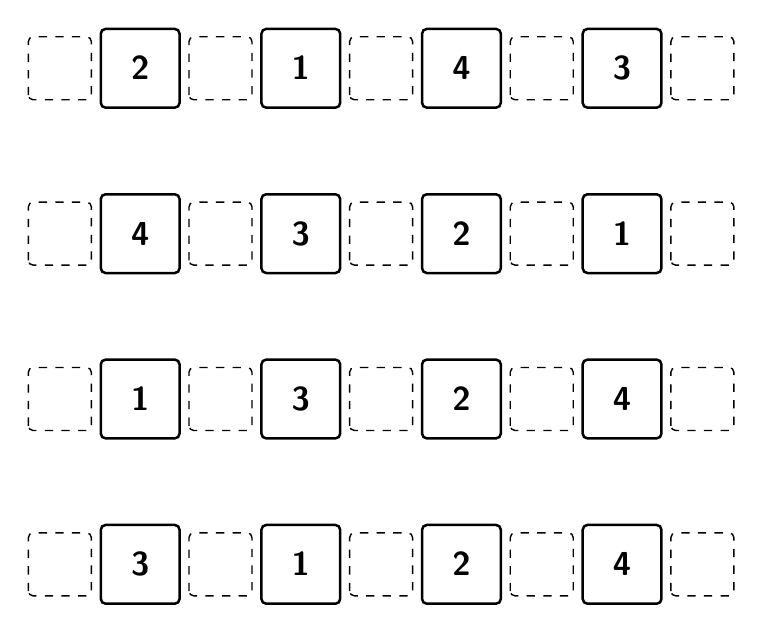
\begin{tikzpicture}[x=1mm,y=1mm]
\draw[dashed, line width=0.5pt, rounded corners=0.6mm] (0,1) rectangle (8,9);
\draw[line width=0.9pt, fill=white, rounded corners=0.6mm] (9.2,0) rectangle (19.2,10);
\node at (14.2,5) {\bfseries\large 2};
\draw[dashed, line width=0.5pt, rounded corners=0.6mm] (20.4,1) rectangle (28.4,9);
\draw[line width=0.9pt, fill=white, rounded corners=0.6mm] (29.6,0) rectangle (39.6,10);
\node at (34.6,5) {\bfseries\large 1};
\draw[dashed, line width=0.5pt, rounded corners=0.6mm] (40.8,1) rectangle (48.8,9);
\draw[line width=0.9pt, fill=white, rounded corners=0.6mm] (50,0) rectangle (60,10);
\node at (55,5) {\bfseries\large 4};
\draw[dashed, line width=0.5pt, rounded corners=0.6mm] (61.2,1) rectangle (69.2,9);
\draw[line width=0.9pt, fill=white, rounded corners=0.6mm] (70.4,0) rectangle (80.4,10);
\node at (75.4,5) {\bfseries\large 3};
\draw[dashed, line width=0.5pt, rounded corners=0.6mm] (81.6,1) rectangle (89.6,9);
\draw[dashed, line width=0.5pt, rounded corners=0.6mm] (0,-20) rectangle (8,-12);
\draw[line width=0.9pt, fill=white, rounded corners=0.6mm] (9.2,-21) rectangle (19.2,-11);
\node at (14.2,-16) {\bfseries\large 4};
\draw[dashed, line width=0.5pt, rounded corners=0.6mm] (20.4,-20) rectangle (28.4,-12);
\draw[line width=0.9pt, fill=white, rounded corners=0.6mm] (29.6,-21) rectangle (39.6,-11);
\node at (34.6,-16) {\bfseries\large 3};
\draw[dashed, line width=0.5pt, rounded corners=0.6mm] (40.8,-20) rectangle (48.8,-12);
\draw[line width=0.9pt, fill=white, rounded corners=0.6mm] (50,-21) rectangle (60,-11);
\node at (55,-16) {\bfseries\large 2};
\draw[dashed, line width=0.5pt, rounded corners=0.6mm] (61.2,-20) rectangle (69.2,-12);
\draw[line width=0.9pt, fill=white, rounded corners=0.6mm] (70.4,-21) rectangle (80.4,-11);
\node at (75.4,-16) {\bfseries\large 1};
\draw[dashed, line width=0.5pt, rounded corners=0.6mm] (81.6,-20) rectangle (89.6,-12);
\draw[dashed, line width=0.5pt, rounded corners=0.6mm] (0,-41) rectangle (8,-33);
\draw[line width=0.9pt, fill=white, rounded corners=0.6mm] (9.2,-42) rectangle (19.2,-32);
\node at (14.2,-37) {\bfseries\large 1};
\draw[dashed, line width=0.5pt, rounded corners=0.6mm] (20.4,-41) rectangle (28.4,-33);
\draw[line width=0.9pt, fill=white, rounded corners=0.6mm] (29.6,-42) rectangle (39.6,-32);
\node at (34.6,-37) {\bfseries\large 3};
\draw[dashed, line width=0.5pt, rounded corners=0.6mm] (40.8,-41) rectangle (48.8,-33);
\draw[line width=0.9pt, fill=white, rounded corners=0.6mm] (50,-42) rectangle (60,-32);
\node at (55,-37) {\bfseries\large 2};
\draw[dashed, line width=0.5pt, rounded corners=0.6mm] (61.2,-41) rectangle (69.2,-33);
\draw[line width=0.9pt, fill=white, rounded corners=0.6mm] (70.4,-42) rectangle (80.4,-32);
\node at (75.4,-37) {\bfseries\large 4};
\draw[dashed, line width=0.5pt, rounded corners=0.6mm] (81.6,-41) rectangle (89.6,-33);
\draw[dashed, line width=0.5pt, rounded corners=0.6mm] (0,-62) rectangle (8,-54);
\draw[line width=0.9pt, fill=white, rounded corners=0.6mm] (9.2,-63) rectangle (19.2,-53);
\node at (14.2,-58) {\bfseries\large 3};
\draw[dashed, line width=0.5pt, rounded corners=0.6mm] (20.4,-62) rectangle (28.4,-54);
\draw[line width=0.9pt, fill=white, rounded corners=0.6mm] (29.6,-63) rectangle (39.6,-53);
\node at (34.6,-58) {\bfseries\large 1};
\draw[dashed, line width=0.5pt, rounded corners=0.6mm] (40.8,-62) rectangle (48.8,-54);
\draw[line width=0.9pt, fill=white, rounded corners=0.6mm] (50,-63) rectangle (60,-53);
\node at (55,-58) {\bfseries\large 2};
\draw[dashed, line width=0.5pt, rounded corners=0.6mm] (61.2,-62) rectangle (69.2,-54);
\draw[line width=0.9pt, fill=white, rounded corners=0.6mm] (70.4,-63) rectangle (80.4,-53);
\node at (75.4,-58) {\bfseries\large 4};
\draw[dashed, line width=0.5pt, rounded corners=0.6mm] (81.6,-62) rectangle (89.6,-54);
\end{tikzpicture}
\end{center}

\par\vspace{3pt}\noindent\begin{tikzpicture}[x=1mm,y=1mm]
\draw[black!30, line width=0.4pt] (0,-9) -- (177,-9);
\draw[black!30, line width=0.4pt] (0,-18) -- (177,-18);
\draw[black!30, line width=0.4pt] (0,-27) -- (177,-27);
\draw[black!30, line width=0.4pt] (0,-36) -- (177,-36);
\end{tikzpicture}\par
\vspace{2pt}
\problem{7}How many of the 120 trains with cars 1, 2, 3, 4, 5 can leave in order? Explain how you know your count is right.
\par\vspace{3pt}\noindent\begin{tikzpicture}[x=1mm,y=1mm]
\draw[black!30, line width=0.4pt] (0,-9) -- (177,-9);
\draw[black!30, line width=0.4pt] (0,-18) -- (177,-18);
\draw[black!30, line width=0.4pt] (0,-27) -- (177,-27);
\draw[black!30, line width=0.4pt] (0,-36) -- (177,-36);
\draw[black!30, line width=0.4pt] (0,-45) -- (177,-45);
\draw[black!30, line width=0.4pt] (0,-54) -- (177,-54);
\draw[black!30, line width=0.4pt] (0,-63) -- (177,-63);
\draw[black!30, line width=0.4pt] (0,-72) -- (177,-72);
\draw[black!30, line width=0.4pt] (0,-81) -- (177,-81);
\end{tikzpicture}\par
\end{document}
